\documentclass{standalone}
\usepackage{tikz}
\usepackage{ctex,siunitx}
\setCJKmainfont{Noto Serif CJK SC}
\usepackage{tkz-euclide}
\usepackage{amsmath}
\usetikzlibrary{patterns, calc}
\usetikzlibrary {decorations.pathmorphing, decorations.pathreplacing, decorations.shapes,}
\begin{document}
\small
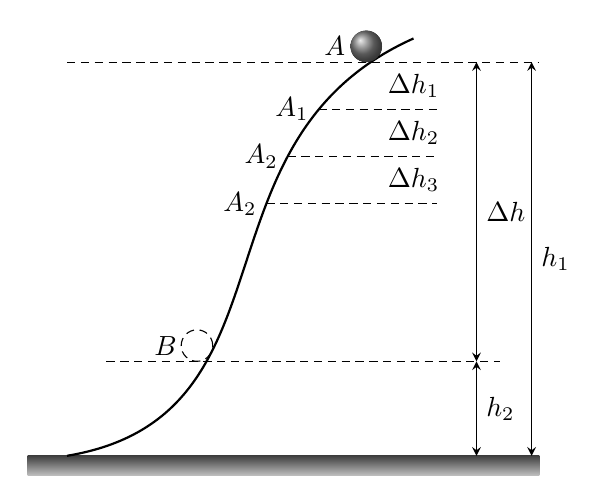
\begin{tikzpicture}[>=stealth,scale=1.0]
  \fill[top color=darkgray,bottom color=lightgray](-3,0)rectangle(3.5,-0.25);
  \draw[thin,densely dashed] (-2.5,5)--(3.5,5)(-2.0,1.2)--(3,1.2);
  \draw[thick](-2.5,0)..controls(0.5,0.5)and(-1.0,4)..(1.9,5.3);
  \fill[ball color=gray](1.30,5.2)circle(0.2);
  \draw[thin,densely dashed](-0.85,1.4)circle(0.2);
  \draw[thin,densely dashed](0.69,4.4)node[left]{$A_1$}--(2.2,4.4)(0.3,3.8)node[left]{$A_2$}--(2.2,3.8)(0.03,3.2)node[left]{$A_2$}--(2.2,3.2);
  \draw[<->,thin](3.4,5)--(3.4,0)node[midway,right]{$h_1$};
  \draw[<->,thin](2.7,5)--(2.7,1.2)node[midway,right]{$\Delta h$};
  \draw[<->,thin](2.7,0)--(2.7,1.2)node[midway,right]{$h_2$};
  \node at (1.9,4.7){$\Delta h_1$};
  \node at (1.9,4.1){$\Delta h_2$};
  \node at (1.9,3.5){$\Delta h_3$};
  \node at (0.9,5.2){$A$};
  \node at (-1.25,1.4){$B$};
\end{tikzpicture}
\end{document}